%!TEX root = ../../main.tex

\chapter{Implementierung und Verbesserung der Webseite}
\label{chapter:6}

In den vorherigen Kapiteln wurde zunächst die bisherige Webseite analysiert, um ihre Stärken und Schwächen zu identifizieren.
Anschließend wurde eine Nutzerumfrage durchgeführt, um die Zufriedenheit der NutzerInnen mit der Webseite zu ermitteln.
Darauf aufbauend wurden aus den Ergebnissen der Nutzerumfrage Personas erstellt und Anforderungen abgeleitet.
Diese Anforderungen wurden im \hyperref[chapter:5]{Kapitel 5} spezifiziert und in die Kategorien Muss-, Soll- und Kann-Anforderungen eingeteilt.

Diese Erkenntnisse sollen nun genutzt werden, um eine verbesserte Version der Webseite zu entwickeln.
Bevor dies geschehen kann, muss jedoch die bisherige Codebasis auf ein neues Frontend-Framework migriert werden, da die Zufriedenheit mit dem vorherigen Framework nicht sehr hoch war.
Nach der Migration werden trotzdem die Ergebnisse der Nutzerumfrage genutzt, um die Webseite zu optimieren.
Dabei wird auf die Ergebnisse der Umfrage eingegangen, und die Webseite wird entsprechend angepasst, um die Nutzererfahrung zu verbessern.
Außerdem werden neue Features und Funktionen hinzugefügt, die die Nutzererfahrung bereichern und die NutzerInnen dazu anregen sollen, die Webseite vermehrt zu nutzen.

Bei jedem relevanten Kapitel werden die entsprechenden Anforderungen, welche dadurch Erfüllt werden, referenziert.
Dadurch, dass manche Anforderungen keine explizite Umsetzung erfordern, da diese in jedem Implemtierungsschritt beachtet werden sollten, werden diese durch das Projekt hinweg konstant betrachtet.
Folgende Anforderungen werden konstant beachtet und angewendet:

\begin{enumerate}

    \item \textbf{[R08] Integration von Grafiken}
    \item \textbf{[R10] Modernisierung des Designs}
    \item \textbf{[R12] Benutzerfreundlichkeit}
    \item \textbf{[R13] Modernes Design}
    \item \textbf{[R14] Zuverlässigkeit}
    \item \textbf{[R15] Wartbarkeit und Erweiterbarkeit}
    \item \textbf{[R16] Code Qualität und Styleguide Einhaltung}

\end{enumerate}

\section{Frameworkwechsel und Verbesserungen}

\subsection{Motivation für den Frameworkwechsel}

Die Webseite wurde bisher unter Verwendung des Frontend-Frameworks \textbf{React.js} entwickelt, das aufgrund seiner Beliebtheit bei vielen Entwicklern weit verbreitet ist.
Dennoch wurde die Entscheidung getroffen, das Framework zu wechseln, bedingt durch verschiedene Herausforderungen und auch aufgrund von Kompetenzüberlegungen der Entwickler.
Durch den Übergang zu einem anderen Framework soll die Webentwicklung vereinfacht und die Nutzererfahrung verbessert werden.
Insbesondere sollen bekannte Probleme wie fehlerhaftes State Management vermieden werden.

Wie bereits im \hyperref[chapter:3-frontend-frameworks]{Grundlagenkapitel} erläutert, wird als neue Framework \textbf{Vue} eingeführt, dass ebenfalls weit verbreitet ist und von vielen Entwicklern genutzt wird.

\subsection{Umsetzung des Frameworkwechsels}

Die Umsetzung ist dabei zunächst nicht zu kompliziert, da das gesamte Projekt in verschiedene Abschnitte unterteilt war, wie zum Beispiel das Frontend der Webseite, das Backend und die Datenbank.
Somit musste lediglich der Ordner, der das Frontend beinhaltet, ausgetauscht werden.
Das Backend und die Datenbank blieben unverändert.
Um das Frontend mit dem neuen Framework (\textbf{Vue}) auszustatten, muss zunächst der Inhalt des bisherigen Ordners, der das Frontend beinhaltet, gelöscht werden.
Daraufhin konnte über das Werkzeug \textbf{Vite} ein \textbf{Vue}-Projekt erstellt werden, dass auch direkt \textbf{TypeScript} unterstützt.
Dies hilft beim Entwickeln schon frühzeitig Probleme zu entdecken und zu lösen.
Im folgenden Code-Snippet ist zu sehen, wie das Projekt mit \textbf{Vite} erstellt wurde.

\begin{lstlisting}[language={bash}, caption={Initialisierung des Vue Projektes mit Vite \cite{vitejs-getting-started}}]
npm create vite@latest
\end{lstlisting}

Nachdem das Projekt erstellt wurde, konnte der Inhalt des Projekts in den alten und leeren Ordner kopiert werden. Danach mussten lediglich noch Konfigurationen angepasst werden, ebenso wie Dockerfiles und Docker Compose. Die Konfigurationen betreffen das \textbf{TypeScript}- und \textbf{Vue}-Projekt, während die Dockerfiles und Docker Compose für die Containerisierung der Webseite zuständig sind. Die entsprechenden Konfigurationen und Dockerfiles sind im folgenden Code Snippet zu sehen.

\begin{lstlisting}[language={bash}, caption={Dockerfile für das Vue Projekt}]
# Use the official Node.js image as the base image
FROM node:16

# Set the working directory inside the container
WORKDIR /usr/src/app

# Copy only the package.json and package-lock.json files to leverage Docker cache
COPY package.json ./
COPY package-lock.json ./

# Install dependencies
RUN npm install

# Copy the entire project files to the container
COPY ./ ./

# Expose the port that the Vue app will run on (change this if your app uses a different port)
EXPOSE 3000

# Build the Vue project
RUN npm run build

# Command to start the Vue app
CMD ["npm", "run", "start"]
\end{lstlisting}

In der Docker Compose-Datei wird der Container für das Vue-Projekt erstellt und konfiguriert. Hierbei muss dann noch explizit der Port angegeben werden, auf dem die Webseite laufen soll.

\begin{lstlisting}[language={bash}, caption={Docker Compose für das Vue Projekt}]
version: "3.8"

client:
stdin_open: true
environment:
    - WDS_SOCKET_PORT=3050
    - CHOKIDAR_USEPOLLING=true
    - WATCHPACK_POLLING=true
build:
    dockerfile: Dockerfile
    context: ./client
volumes:
    - /app/node_modules
    - ./client:/app
ports:
    - "3000:3000"
\end{lstlisting}

Das alles funktioniert reibungslos. Außerdem muss in der \texttt{vite.config.ts}-Datei noch der Port angepasst werden, auf dem die Webseite laufen soll. Dieser muss mit dem Port in der Docker-Compose-Datei übereinstimmen.

\begin{lstlisting}[language={JavaScript}, caption={Port Konfiguration für das Vue Projekt}]
export default defineConfig({
    ...
    server: {
    host: '0.0.0.0',
    port: 3000,
},
});
\end{lstlisting}

Nach diesem Schritt ist das Projekt erfolgreich migriert und kann nun mit dem neuen Framework weiterentwickelt werden. Es ist auch möglich, alles über die Docker Compose Datei zu starten und zu stoppen.

\section{Unterstützung von PWA für Mobile NutzerInnen}

Zu Beginn dieser Arbeit wurde in \hyperref[chapter:2]{Kapitel 2} erwähnt, dass die Webseite trotz ihrer webbasierten Natur als App bezeichnet wird.
Um die Nutzererfahrung zu optimieren und die Benutzerfreundlichkeit der Webseite zu erhöhen, wird die Integration von \acf{PWA} angestrebt.
Eine \acs{PWA} ist eine Technologie, die es ermöglicht, Webseiten ähnlich wie native Mobile Apps zu nutzen.
Dies bedeutet, dass die Webseite auch offline zugänglich ist und auf dem Startbildschirm eines Smartphones installiert werden kann.
Dadurch wird die Interaktion mit der Webseite komfortabler und die Nutzererfahrung insgesamt verbessert. \cite{ms-pwa}

Die Implementierung von \acs{PWA} gestaltet sich vergleichsweise unkompliziert und erfordert nur wenige Schritte. Zunächst wird ein Plugin zu Vite hinzugefügt, das sich um die \acs{PWA}-Funktionalität kümmert. Dies kann einfach über die Konsole durch die Installation des entsprechenden Plugins erfolgen.

\begin{lstlisting}[language={bash}, caption={Installation des PWA Plugins}]
npm i vite-plugin-pwa -D 
\end{lstlisting}

Danach müssen wir die Vite-Konfiguration anpassen, um das Plugin zu aktivieren und zu konfigurieren.
Dies umfasst das Hinzufügen eines Manifests, eines Service Workers, sowie verschiedener Grafiken für mobile Geräte.
Im folgenden Code-Snippet wird dargestellt, wie die Vite-Konfiguration angepasst wurde, um die Unterstützung für \acs{PWA} zu integrieren.

\begin{lstlisting}[language={JavaScript}, caption={Angepasste Vite Konfiguration für PWA}]
...
import { VitePWA } from 'vite-plugin-pwa';

export default defineConfig({
    plugins: [
        ...
        VitePWA({
            registerType: 'autoUpdate',
            devOptions: {
                enabled: true,
            },
            includeAssets: [
                'favicon.ico',
                'apple-touch-icon.png',
                'mask-icon.svg',
            ],
            manifest: {
                name: 'CO2Runter',
                short_name: 'CO2Runter',
                description:
                    'CO2 Runter Webseite hilft bei der Reduktion von CO2',
                theme_color: '#ffffff',
                icons: [
                    {
                        src: '/pwa-192x192.png',
                        sizes: '192x192',
                        type: 'image/png',
                    },
                    {
                        src: '/pwa-512x512.png',
                        sizes: '512x512',
                        type: 'image/png',
                    },
                    {
                        src: '/pwa-512x512.png',
                        sizes: '512x512',
                        type: 'image/png',
                        purpose: 'any maskable',
                    },
                ],
            },
        }),
    ],
    ...
});
\end{lstlisting}

Ebenfalls erfordert es die Anpassung der \texttt{index.html}-Datei, um die im Manifest definierten Grafiken zu laden.

\begin{lstlisting}[language={JavaScript}, caption={Anpassungen an der index.html Datei}]
<!DOCTYPE html>
<html lang="en">

<head>
    <meta charset="UTF-8" />
    <meta name="viewport" content="width=device-width, initial-scale=1.0" />
    <title>CO2 Runter</title>
    <meta name="description" content="CO2 Runter Webseite hilft bei der Reduktion von CO2">

    <link rel="icon" href="/favicon.ico">
    <link rel="apple-touch-icon" href="/apple-touch-icon.png" sizes="180x180">
    <link rel="mask-icon" href="/mask-icon.svg" color="#FFFFFF">
    <meta name="theme-color" content="#ffffff">
</head>

<body>
    <div id="app"></div>
    <script type="module" src="/src/main.ts"></script>
</body>

</html>
\end{lstlisting}

Das Manifest ist eine \acf{JSON}-Datei, die im Hintergrund von Vite generiert wird und Informationen über die Webseite enthält, wie den Namen, die Beschreibung, das Icon und die Farbe. Der Service Worker ist ein Skript, das im Hintergrund ausgeführt wird und die Offline-Funktionalität der App ermöglicht. Nun ist die Webseite als \acs{PWA} konfiguriert und kann auf dem Homescreen des Smartphones installiert werden. Um dies zu erleichtern, kann eine Komponente erstellt werden, die den NutzerInnen dazu auffordert, die Webseite zu installieren. Diese könnte wie folgt aussehen:

\begin{lstlisting}[language={JavaScript}, caption={PWA Vue Komponente}]
<script setup lang="ts">
import { onBeforeMount, ref } from 'vue';

const deferredPrompt = ref<any>(null);

const beforeInstallPromptHandler = (e: Event) => {
    e.preventDefault();
    deferredPrompt.value = e;
};

const appInstalledHandler = () => {
    deferredPrompt.value = null;
};

onBeforeMount(() => {
    window.addEventListener('beforeinstallprompt', beforeInstallPromptHandler);
    window.addEventListener('appinstalled', appInstalledHandler);
});

const dismiss = () => {
    deferredPrompt.value = null;
};

const install = () => {
    if (deferredPrompt.value) {
        deferredPrompt.value.prompt();
    }
};
</script>

<template>
    <v-alert
        v-if="deferredPrompt"
        icon="mdi-download"
        color="info"
        title="Alert title"
        text="Lorem ipsum dolor sit amet consectetur adipisicing elit. Commodi, ratione debitis quis est labore voluptatibus! Eaque cupiditate minima, at placeat totam, magni doloremque veniam neque porro libero rerum unde voluptatem!"
    >
        <br />
        <v-btn @click="dismiss">Dismiss</v-btn>
        <v-btn @click="install">Install</v-btn>
    </v-alert>

    <v-banner
        v-if="deferredPrompt"
        lines="one"
        icon="mdi-download"
        color="info"
    >
        <template v-slot:text>
            Willst du diese Webseite installieren?
        </template>

        <template v-slot:actions>
            <v-btn @click="dismiss">Nein</v-btn>
            <v-btn @click="install">Ja, installieren</v-btn>
        </template>
    </v-banner>
</template>

\end{lstlisting}

Die Integration dieser Komponente in die \texttt{App.vue}-Datei ist unkompliziert und wird dem NutzerInnen angezeigt, wenn die Webseite als \acs{PWA} installiert werden kann. Dadurch wird die Nutzererfahrung verbessert und die Webseite kann auch offline genutzt werden, ähnlich wie eine native App. \cite{vite-plugin-pwa}

\section{Projekt aufräumen und Strukturierung}

Bisher wurden essentielle Veränderungen an dem Framework gemacht.
Bevor es weitergeht, muss das Projekt aufgeräumt und strukturiert werden.
Dies beinhaltet das Entfernen von ungenutzten Dateien und das Umbenennen von Dateien, um eine konsistente Namenskonvention zu gewährleisten.
Außerdem müssen die Ordnerstruktur und die Dateistruktur überarbeitet werden, um eine bessere Übersichtlichkeit und Wartbarkeit des Projekts zu gewährleisten.
Dies beinhaltet das Erstellen von Ordnern für Komponenten, Seiten, Services und anderen wichtigen Dateien.
Die Ordnerstruktur könnte wie folgt aussehen:

% TODO: Ordnerstruktur demonstrieren

\section{Erstellung der neuen Landing Page}

Die Landing Page ist die erste Seite, die der NutzerInnen sieht, wenn er die Webseite besucht.
Sie ist somit das Aushängeschild der Webseite und sollte den NutzerInnen dazu animieren, die Webseite zu nutzen.
Die Landing Page sollte also ansprechend und informativ sein, um den NutzerInnen zu überzeugen, die Webseite zu nutzen als auch die zuvor definierte Anforderung \textbf{[R04]} erfüllen.
Die neue Landing Page wird mit \textbf{Vuetify} erstellt, einem Material Design Framework für Vue.js.
Vuetify bietet viele vorgefertigte Komponenten, die es ermöglichen, schnell und einfach ansprechende Webseiten zu erstellen.
Die Landing Page könnte wie folgt aussehen:

\begin{figure}[H]
    \centering
    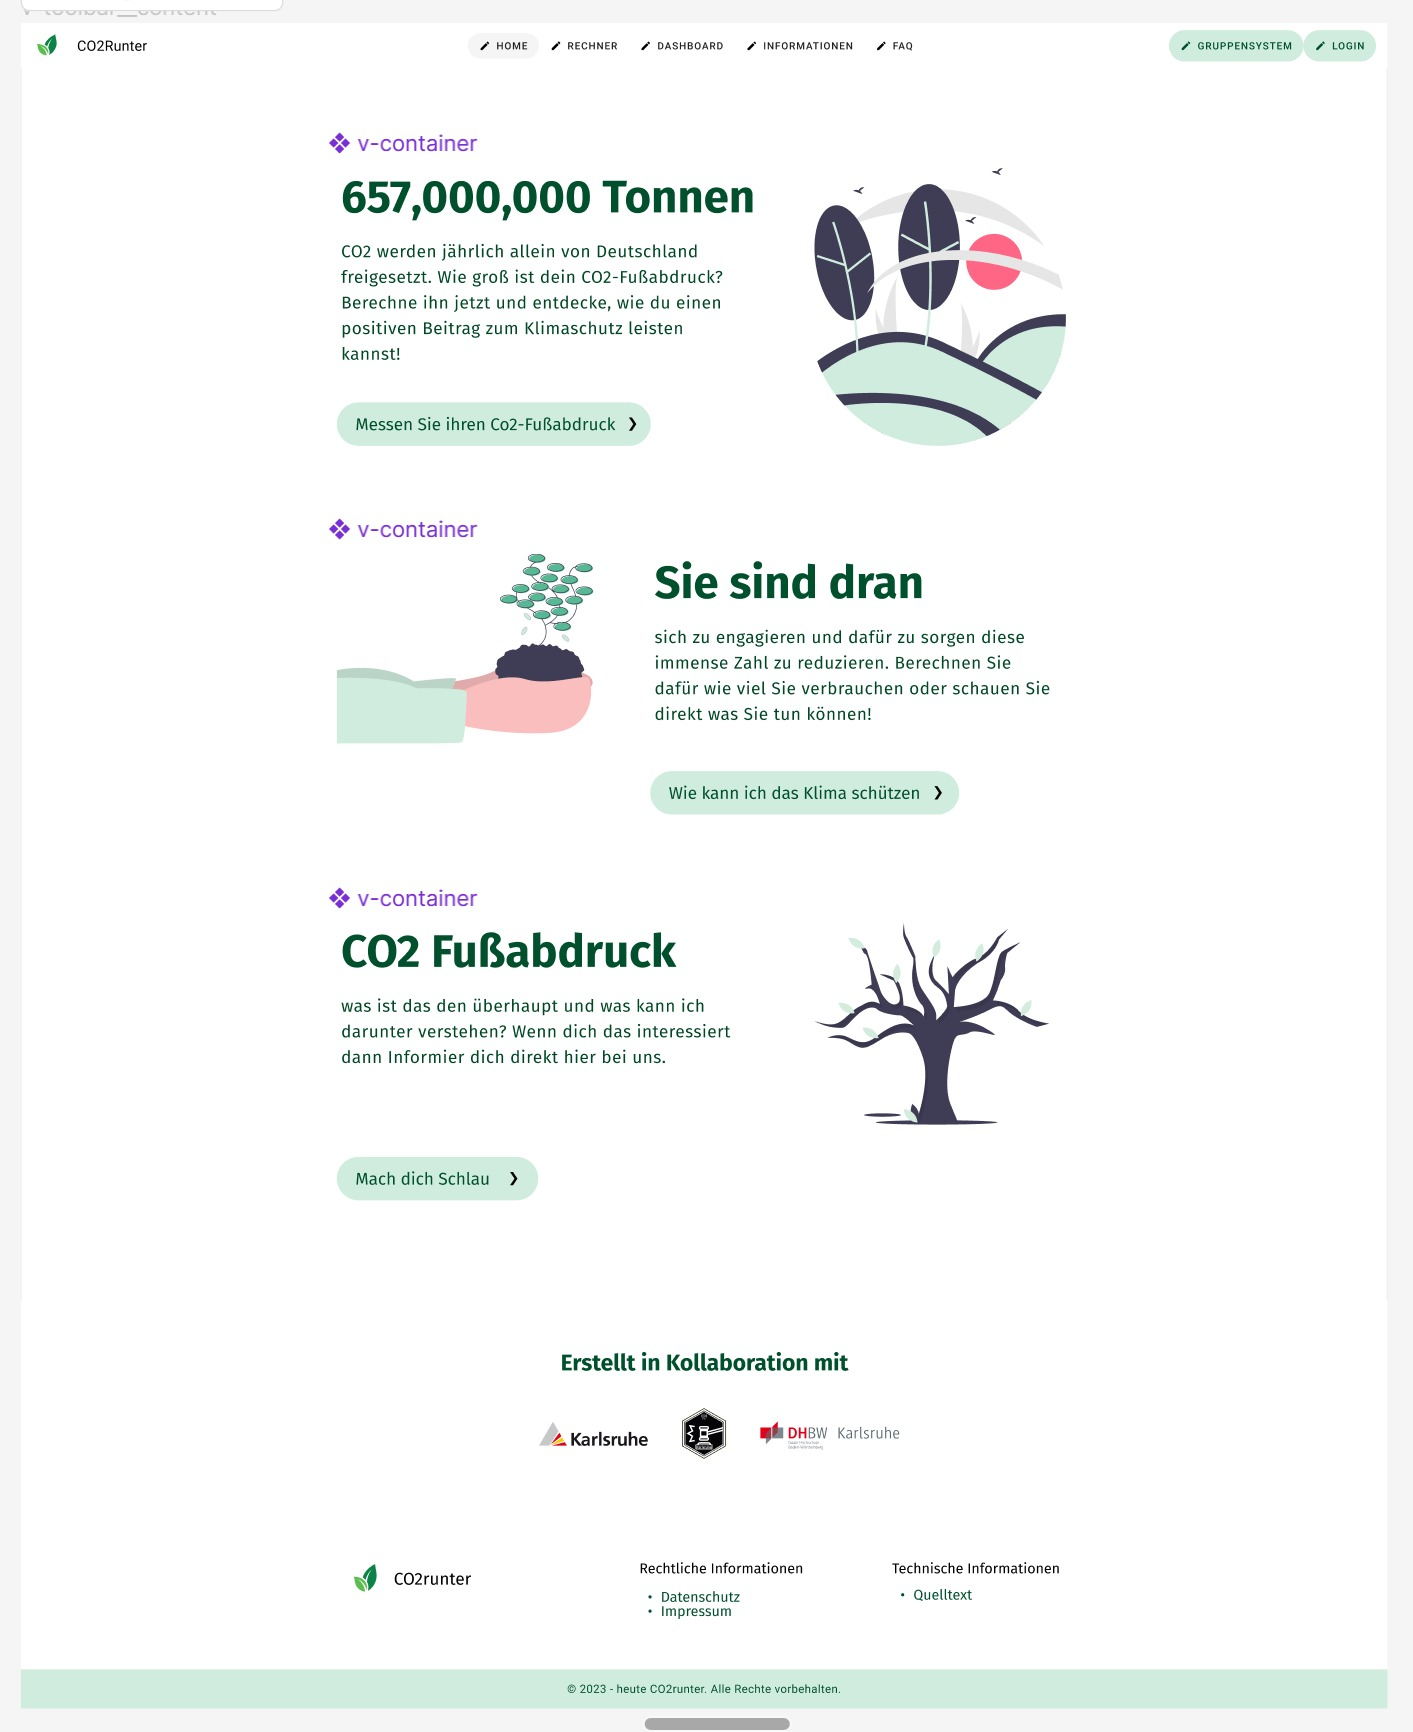
\includegraphics[width=0.8\textwidth]{images/06/HomePage-Design.jpeg}
    \caption{Das neu erstelle CO2-Runter Design der Landigpage anhand der nuterzentrierten Umfrage}
    \label{fig:new-co2runter-homepage-design}
\end{figure}

Das Design, welches in der \hyperref[fig:new-co2runter-homepage-design]{vorheriger Abbildung} zu sehen war, wurde anhand der Evaluierung der Umfrage und der erstellten Personas erstellt.
Dafür wurde das Tool Figma genutzt und auch direkt mit Vuetify Komponenten gearbeitet, wodurch die Entwicklungsarbeitszeit immens verkürzt wurde.
Das ist deshalb der Fall, da das Design und die Komponenten im späteren Implementierungsverlauf 1:1 übernommen werden konnten.

Die neue Homepage kann man in drei Sektionen unterteilen.
Einmal die Navigationsleiste, den Kontent der Landing Page und den Footer mit desen relevanten Informationen.
Zu beachten ist hierbei das die Navigationsleiste, als auch der Footer, auf allen Seiten identisch sein sollen.
Einzig der Kontent einer Seite ist dynamisch und soll deshalb veränderbar sein.
Daher werden die drei Sektionen im folgenden nacheinander durchgearbeitet.
Zuvor aber werden wichtige Änderungen vorgenommen.

\subsection{Änderungen}

Eine wichtige Änderung ist die Anpassung des Farbschemas, um die Webseite ansprechender zu gestalten. Dafür wird das Farbschema von Vuetify angepasst, um eine konsistente Farbgebung zu gewährleisten. Hierfür erstellen wir lediglich nach der Vuetify dokumentation ein neues Farbschema und passen die Farben an. Dieses Farbschema wird dann in der Vuetify Konfiguration eingebunden. Das Farbschema sieht dann wie folgt aus: \cite{vuetiy-custom-color-theme}

\begin{lstlisting}[language={JavaScript}, caption={Vuetify Farbschema anpassung}]
const customLightTheme = {
    dark: false,
    colors: {
        background: '#FFFFFF',
        surface: '#FFFFFF',
        'surface-bright': '#FFFFFF',
        'surface-light': '#EEEEEE',
        'surface-variant': '#424242',
        'on-surface-variant': '#EEEEEE',
        primary: '#D0ECDE',
        'primary-darken-1': '#01502D',
        secondary: '#004725',
        'secondary-darken-1': '#018786',
        error: '#B00020',
        info: '#2196F3',
        success: '#4CAF50',
        warning: '#FB8C00',
    },
    variables: {
        'border-color': '#000000',
        'border-opacity': 0.12,
        'high-emphasis-opacity': 0.87,
        'medium-emphasis-opacity': 0.6,
        'disabled-opacity': 0.38,
        'idle-opacity': 0.04,
        'hover-opacity': 0.04,
        'focus-opacity': 0.12,
        'selected-opacity': 0.08,
        'activated-opacity': 0.12,
        'pressed-opacity': 0.12,
        'dragged-opacity': 0.08,
        'theme-kbd': '#212529',
        'theme-on-kbd': '#FFFFFF',
        'theme-code': '#F5F5F5',
        'theme-on-code': '#000000',
    },
};

export default createVuetify({
    theme: {
        defaultTheme: 'customLightTheme',
        themes: {
            customLightTheme,
        },
    },
});
\end{lstlisting}

Nicht nur die Farben, sondern auch das Layout sollte angepasst werden.
Dafür wird ein Layout erstellt, welches auf allen Seiten gleich ist und nur der Kontent variabel ist.
Dieses Layout wird dann in jeder Seite durch die Vue Router Funktionalität eingebunden.
Das Einbinden sieht wie folgt aus:

\begin{lstlisting}[language={JavaScript}, caption={Einbindung des Layouts in der Vue Router Konfiguration}]
const routes = [
    {
        path: '/',
        component: () => import('@/layouts/default/Default.vue'),
        children: [
            {
                path: '',
                name: 'Home',
                component: () => import('@/views/HomeView.vue'),
            },
        ],
    },
    ...
];
\end{lstlisting}

Damit das Einbinden richtig funktioniert, muss in der \texttt{Default.vue} Datei mindestens ein \texttt{<router-view />} Tag existieren, damit die jeweilige Seite eingebunden und angezeigt wird.
Das angepasste Layout der CO2-Runter-Webseite beinhaltet, dass auf jeder erreichbaren Seite die Navigationsleiste, der Kontent und der Footer angezeigt wird.
Dieses Layout wird dann in der \texttt{App.vue} Datei wiederum über ein \texttt{<router-view />} Tag eingebunden und sieht wie folgt aus:

\begin{lstlisting}[language={JavaScript}, caption={Layout Definition}]
<template>
    <v-locale-provider>
        <v-app>
            <TheNavigationHeader />
            <v-main>
                <v-divider />
                <v-container :fluid="true" class="page-wrapper">
                    <div class="maxWidth">
                        <RouterView />
                    </div>
                </v-container>
            </v-main>
            <TheFooter />
        </v-app>
    </v-locale-provider>
</template>
\end{lstlisting}

Nachdem diese Schritte befolgt wurden und jede Seite das Layout eingebunden hat, sowie das Farbschema zu jeder Webseite angepasst wurde, kann sich nun um die restliche Komponenten gekümmert werden.
Dabei handelt es sich um die Komponenten der Navigationsleiste, des Kontents und des Footers.

\subsection{Navigationsleiste}

Eine Navigationsleiste dient dem NutzerInnen einer Webseite dazu, den Überblick über den aktuell zu sehenden Bereich einer Webseite zu behalten und biete eine schnelle und einfache Navigation über die Webseite.
Im Fall der CO2-Runter-App gibt es die Startseite, den CO2-Rechner, das Dashboard, sowie eine FAQ- und Gruppensystemseite.
Diese sollen über die Navigationsleiste erreichbar sein.
Die folgende Abbildung zeigt, wie die Navigationsleiste implementiert wurde:

\begin{lstlisting}[language={JavaScript}, caption={Navigationsleiste für Web als auch Mobile}]
<template>
    <v-app-bar :elevation="0">
        <v-app-bar-nav-icon
            class="hidden-md-and-up ms-md-3 ms-sm-5 ms-3 text-muted"
            @click.capture="isDrawerOpen = !isDrawerOpen"
        ></v-app-bar-nav-icon>

        <v-toolbar-title>
            <v-list class="d-flex">
                <v-list-item
                    to="/"
                    :exact="true"
                    title="CO2Runter"
                    class="rounded-lg"
                    prepend-avatar="../assets/co2runter-logo.png"
                    color="primary-darken-1"
                />
            </v-list>
        </v-toolbar-title>

        <div class="hidden-sm-and-down">
            <v-list class="d-flex">
                <v-list-item
                    to="/co2Rechner"
                    title="CO2 Rechner"
                    prepend-icon="mdi-calculator-variant-outline"
                    class="mx-1 rounded-lg"
                    color="primary-darken-1"
                />

                <v-list-item
                    to="/dashboard"
                    title="Dashboard"
                    prepend-icon="mdi-view-dashboard-outline"
                    class="mx-1 rounded-lg"
                    color="primary-darken-1"
                />

                <v-list-item
                    to="/faq"
                    title="FAQ"
                    prepend-icon="mdi-frequently-asked-questions"
                    class="mx-1 rounded-lg"
                    color="primary-darken-1"
                />

                <v-list-item
                    to="/gruppensystem"
                    :exact="true"
                    title="Gruppensystem"
                    prepend-icon="mdi-account-group-outline"
                    class="mx-1 rounded-lg"
                    color="primary-darken-1"
                />

                <v-list-item
                    v-if="!isLoggedIn"
                    to="/login-registration"
                    :exact="true"
                    title="Login"
                    prepend-icon="mdi-login-variant"
                    class="rounded-lg mx-1 mr-3"
                    color="primary-darken-1"
                    :active="true"
                />

                <v-menu v-else :close-on-content-click="false">
                    <template v-slot:activator="{ props }">
                        <v-list-item
                            v-bind="props"
                            class="rounded-lg mx-1 mr-3"
                            color="primary-darken-1"
                            :active="true"
                        >
                            <template v-slot:prepend>
                                <v-icon>mdi-account</v-icon>
                            </template>

                            <v-list-item-title>Konto </v-list-item-title>

                            <template v-slot:append>
                                <v-icon>mdi-unfold-more-horizontal</v-icon>
                            </template>
                        </v-list-item>
                    </template>

                    <v-sheet rounded="lg" elevation="10" class="mt-2">
                        <v-list class="pa-4">
                            <v-list-subheader>Konto Aktionen </v-list-subheader>

                            <v-list-item
                                title="Gruppen Infos"
                                prepend-icon="mdi-information-outline"
                                class="mb-1 rounded-lg"
                                color="primary-darken-1"
                                to="/gruppensystem/gruppen-informationen"
                            />

                            <v-list-item
                                title="Logout"
                                prepend-icon="mdi-logout"
                                class="mb-1 rounded-lg"
                                color="primary-darken-1"
                                @click="logout()"
                            />
                        </v-list>
                    </v-sheet>
                </v-menu>
            </v-list>
        </div>
    </v-app-bar>

    <v-navigation-drawer v-model="isDrawerOpen" class="hidden-md-and-up">
        <v-divider />

        <v-list class="pa-4">
            <v-list-subheader>Navigation</v-list-subheader>

            <v-list-item
                to="/co2Rechner"
                title="CO2 Rechner"
                prepend-icon="mdi-calculator-variant-outline"
                class="mb-1 rounded-lg"
                color="primary-darken-1"
            />

            <v-list-item
                to="/dashboard"
                title="Dashboard"
                prepend-icon="mdi-view-dashboard-outline"
                class="mb-1 rounded-lg"
                color="primary-darken-1"
            />

            <v-list-item
                to="/faq"
                title="FAQ"
                prepend-icon="mdi-frequently-asked-questions"
                class="mb-1 rounded-lg"
                color="primary-darken-1"
            />

            <v-list-item
                to="/gruppensystem"
                :exact="true"
                title="Gruppensysten"
                prepend-icon="mdi-account-group-outline"
                class="mb-1 rounded-lg"
                color="primary-darken-1"
            />

            <v-list-item
                v-if="!isLoggedIn"
                to="/login-registration"
                :exact="true"
                title="Login"
                prepend-icon="mdi-login-variant"
                class="mb-1 rounded-lg"
                color="primary-darken-1"
                :active="true"
            />

            <v-menu v-else :close-on-content-click="false">
                <template v-slot:activator="{ props }">
                    <v-list-item
                        v-bind="props"
                        class="rounded-lg"
                        color="primary-darken-1"
                        :active="true"
                    >
                        <template v-slot:prepend>
                            <v-icon>mdi-account</v-icon>
                        </template>

                        <v-list-item-title>Konto </v-list-item-title>

                        <template v-slot:append>
                            <v-icon>mdi-unfold-more-horizontal</v-icon>
                        </template>
                    </v-list-item>
                </template>

                <v-sheet rounded="lg" elevation="10" class="mt-2">
                    <v-list class="pa-4">
                        <v-list-subheader>Konto Aktionen </v-list-subheader>

                        <v-list-item
                            title="Gruppen Infos"
                            prepend-icon="mdi-information-outline"
                            class="mb-1 rounded-lg"
                            color="primary-darken-1"
                            to="/gruppensystem/gruppen-informationen"
                        />

                        <v-list-item
                            title="Logout"
                            prepend-icon="mdi-logout"
                            class="mb-1 rounded-lg"
                            color="primary-darken-1"
                            @click="logout()"
                        />
                    </v-list>
                </v-sheet>
            </v-menu>
        </v-list>
    </v-navigation-drawer>

    <PWAInstallationDialog />
</template>
\end{lstlisting}
% TODO: viel zu lang. Muss gekürzt werden.

\subsection{Footer}
Ein Footer ist das Gegenstück zur Navigationsleiste und ist immer ganz am Ende bzw. am unteren Bereich einer Webseite zu finden.
Auch der Footer dient dazu, Informationen darzustellen und besser über eine Webseite navigieren zu können.
Um den Footer zu erzeugen, gibt es drei Bereiche.
Einmal die Logos der Partner, dann die rechtlichen Informationen und die technischen Informationen und an Ende der Copyright.

% TODO: Snippet anpassen!
\begin{lstlisting}[language={JavaScript}, caption={Footer Definition}]
    <template>
    <v-divider />

    <div class="">
        <div class="d-flex justify-center align-center mt-16">
            <h1 class="text-primary-darken-1">Erstellt in Kollaboration</h1>
        </div>

        <v-container class="my-16">
            <v-row
                class="d-flex flex-column flex-md-row justify-center align-center"
                align-content="center"
                :no-gutters="true"
            >
                <v-col class="d-flex justify-center mb-3 mb-md-0">
                    <v-img
                        height="60px"
                        class="clickable-image"
                        src="../../public/images/Logos/Stadtkarlsruhe-logo.svg"
                        @click="navigate('https://www.karlsruhe.de/')"
                    />
                </v-col>
                <v-col class="d-flex justify-center mb-3 mb-md-0">
                    <v-img
                        height="120px"
                        class="clickable-image"
                        src="../../public/images/Logos/CodeFor-karlsruhe.svg"
                        @click="navigate('https://ok-lab-karlsruhe.de/')"
                    />
                </v-col>
                <v-col class="d-flex justify-center">
                    <v-img
                        height="60px"
                        class="clickable-image"
                        src="../../public/images/Logos/dhbw-logo.svg"
                        @click="
                            navigate(
                                'https://www.karlsruhe.dhbw.de/startseite.html'
                            )
                        "
                    />
                </v-col>
            </v-row>
        </v-container>

        <v-divider />

        <v-container class="my-16">
            <v-row justify="center">
                <v-col cols="12" md="4" order-md="1">
                    <v-list class="d-flex">
                        <v-list-item
                            to="/"
                            :exact="true"
                            title="CO2Runter"
                            class="rounded-lg"
                            prepend-avatar="../../public/apple-touch-icon.png"
                            color="primary-darken-1"
                        />
                    </v-list>
                </v-col>
                <v-col cols="12" md="4" order-md="2">
                    <v-list class="pa-4">
                        <v-list-subheader
                            >Rechtliche Informationen
                        </v-list-subheader>

                        <v-list-item
                            href="https://www.karlsruhe.de/datenschutz"
                            title="Datenschutz"
                            prepend-icon="mdi-shield-account-outline"
                            class="mb-1 rounded-lg"
                            color="primary-darken-1"
                        />

                        <v-list-item
                            href="https://www.karlsruhe.de/impressum"
                            title="Impressum"
                            prepend-icon="mdi-text-box-outline"
                            class="mb-1 rounded-lg"
                            color="primary-darken-1"
                        />
                    </v-list>
                </v-col>
                <v-col cols="12" md="4" order-md="2">
                    <v-list class="pa-4">
                        <v-list-subheader
                            >Technische Informationen
                        </v-list-subheader>

                        <v-list-item
                            href="https://github.com/stadt-karlsruhe/CO2-Runter"
                            title="Quelltext"
                            prepend-icon="mdi-file-code-outline"
                            class="mb-1 rounded-lg"
                            color="primary-darken-1"
                        />
                    </v-list>
                </v-col>
            </v-row>
        </v-container>
    </div>

    <v-footer
        class="text-center d-flex justify-center align-center"
        color="primary"
    >
        <div class="text-primary-darken-1">
            2023 - heute | CO2Runter. Alle Rechte vorbehalten.
        </div>
    </v-footer>
</template>
\end{lstlisting}
% TODO: auch zu lang. Auf wesentliches kürzen

\subsection{Kontent}

%TODO: schreiben wir wir den Kontent der Landing Page erstellt haben


% TODO: Snippet anpassen!
\begin{lstlisting}[language={JavaScript}, caption={Home Page Kontent}]
<template>
    <v-container justify="center">
        <v-row class="d-flex flex-column-reverse flex-md-row my-16">
            <v-col cols="12" md="7" class="text-center text-md-start">
                <h1 class="text-primary-darken-1">657,000,000 Tonnen</h1>
                <p class="text-secondary my-8">
                    Text1
                </p>
                <v-btn
                    variant="tonal"
                    :rounded="true"
                    color="primary-darken-1"
                    append-icon="mdi-chevron-right"
                    size="large"
                >
                    Aktion 1
                </v-btn>
            </v-col>
            <v-col class="d-flex align-center justify-center" cols="12" md="5">
                <v-img
                    width="360px"
                    height="200px"
                    src="../assets/undraw_nature_m5ll.svg"
                />
            </v-col>
        </v-row>

        <v-row class="d-flex flex-column flex-md-row my-16">
            <v-col class="d-flex align-center justify-center" cols="12" md="5">
                <v-img
                    width="360px"
                    height="200px"
                    src="../assets/undraw_environment_iaus.svg"
                />
            </v-col>
            <v-col cols="12" md="7" class="text-center text-md-start">
                <h1 class="text-primary-darken-1">Sie sind dran</h1>
                <p class="text-secondary my-8">
                    Text 2
                </p>
                <v-btn
                    variant="tonal"
                    :rounded="true"
                    color="primary-darken-1"
                    append-icon="mdi-chevron-right"
                    size="large"
                >
                    Aktion 2
                </v-btn>
            </v-col>
        </v-row>

        <v-row class="d-flex flex-column-reverse flex-md-row my-16">
            <v-col cols="12" md="7" class="text-center text-md-start">
                <h1 class="text-primary-darken-1">Sie sind dran</h1>
                <p class="text-secondary my-8">
                    Text 3
                </p>
                <v-btn
                    variant="tonal"
                    :rounded="true"
                    color="primary-darken-1"
                    append-icon="mdi-chevron-right"
                    size="large"
                >
                    Aktion 3
                </v-btn>
            </v-col>
            <v-col class="d-flex align-center justify-center" cols="12" md="5">
                <v-img
                    width="360px"
                    height="200px"
                    src="../assets/undraw_waiting__for_you_ldha.svg"
                />
            </v-col>
        </v-row>
    </v-container>
</template>
\end{lstlisting}

\section{Neuerstellung des CO2-Rechners}

% TODO: Anforderung [R19] umsetzen: Question.json anpassen
% TODO: Anforderung [R11] umsetzen: Anzeige von weiteren Quellen/Infos im CO2 Rechner
% TODO: Anforderung [R09] umsetzen: Visualisierung und Vergleich des CO2-Fußabdrucks
% TODO: Anforderung [R07] umsetzen: Durchführung des CO2-Rechner-Workflows
% TODO: Anforderung [R06] umsetzen: Tipps und Tricks zur Reduktion des CO2-Fußabdrucks
% TODO: Anforderung [R03] umsetzen: Hochladen von CO2 Daten
% TODO: Anforderung [R02] umsetzen: Berechnung von CO2 Fußabdruck
% TODO: Anforderung [R01] umsetzen: Abrufen der Bestandsdaten von der Datenbank

Der CO2-Rechner ist ein wichtiges Feature der Webseite, da dem NutzerInnen dadurch ermöglicht wird, seinen CO2-Fußabdruck zu berechnen und Tipps zur Reduzierung zu erhalten.
Bei der Neuerstellung hat man sich an der bisherigen Implementierung orientiert und diese verbessert.

Der CO2-Rechner besteht aus mehreren Kategorien, die der NutzerInnen durchlaufen muss, um seinen CO2-Fußabdruck zu berechnen.
Die Kategorien lauten: Mobilität, Ernährung, Wohnen und Konsum.
Der NutzerInnen muss für jede Kategorie verschiedene Fragen beantworten, um seinen CO2-Fußabdruck zu berechnen.
Die Fragen sind so gestaltet, dass der NutzerInnen sie leicht beantworten kann.
Die Fragen könnten wie folgt aussehen:

\begin{figure}[H]
    \centering
    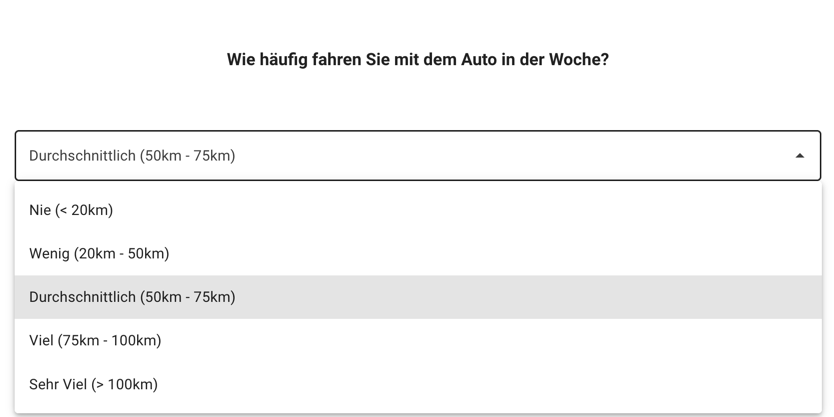
\includegraphics[width=1\textwidth]{images/06/Question_New_Design.png}
    \caption{Design einer Frage des neuen CO2-Rechners}
    \label{fig:new-co2runter-question-design}
\end{figure}

Besonders viel hat sich nicht am Design einer Frage innerhalb des Rechners geändert.
Es wurden jedoch mehr Fragen in den Rechner eingebaut, die im alten Design als "detailliert" beschrieben wurden.
Zusätzlich wurde, wie bereits im Abschnitt
% TODO: Abschnitt mit JSON Veränderung einfügen
, der Wert hinter den Anwortmöglichkeiten angepasst sowie die gesamte Struktur des generierten \acs{JSON}.

Die größte Veränderung erlebt der neue CO2-Rechner in Sachen Allgemeindesign und Nutzerfreundlichkeit.
Wie in Abbildung \ref{fig:new-co2runter-calculator-design} zu sehen ist, wurde hier besonders darauf geachtet, dem NutzerInnen eine ansprechende Webseite zu präsentieren, die nicht nur als langweiliger und stumpfer Fragebogen durchgeht.

\begin{figure}[H]
    \centering
    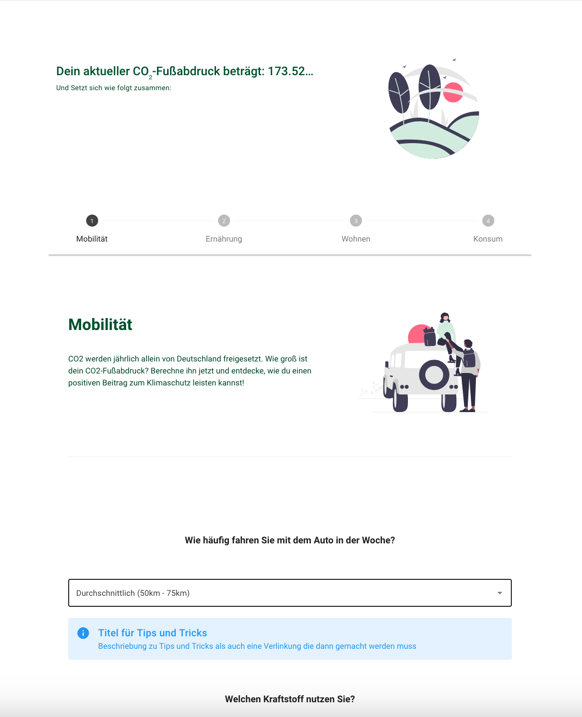
\includegraphics[width=0.8\textwidth]{images/06/Calculator_New_Design.png}
    \caption{Design des neuen CO2-Rechners}
    \label{fig:new-co2runter-calculator-design}
\end{figure}

Der berechnete CO2-Wert aus den gewählten Antwortmöglichkeiten befindet sich nun direkt am Start der Webseite.
Um den berechneten Fußabdruck noch deutlicher in den Vordergrund zu setzen, wurde diesem die Primärfarbe verpasst, so dass er in einem dunkelgrün erscheint.

Eine weitere grundlegende Veränderung des neuen CO2-Rechners findet man unmittelbar unterhalb der Kategorienauflistung.
Bevor der NutzerInnen auf den eigentlichen Rechner stößt, wurde für jede Kategorie ein kleiner Einführungsabschnitt geschrieben und ein dazu passendes Bild hinzugefügt.
Diese Neuerung soll dafür sorgen, dass sich der NutzerInnen nicht direkt in den Rechner stürzt, sondern über das aktuelle Thema aufgeklärt und informiert wird.
Außerdem bringt der Abschnitt mit dem Bild einen positiven Aspekt im Bereich der Nutzerfreundlichkeit.

Für die Implementierung des neuen CO2-Rechner wurde eine neue Komponente namens "CalculatorView.vue" erstellt.
Diese bildet die Hauptansicht des Rechners und implementiert weitere, kleinere Komponenten, so genannte \textit{Components} und ist in der folgenden Abbildung zu sehen.

\begin{lstlisting}[language={JavaScript}, caption={Aufbau der CalculatorView.vue Komponente}]
<template>
    <v-container>
        <v-row
        class= ...
        >
            <v-col ...>
                <CurrentCO2 />
            </v-col>
            <v-col ... >
                <v-img
                width="360px"
                height="200px"
                src="../assets/undraw_nature_m5ll.svg"
                />
            </v-col>
        </v-row>

        <v-row ... >
            <v-col>
                <QuestionStepper />
            </v-col>
        </v-row>
    </v-container>
</template>
\end{lstlisting}

Wie bereits eingangs erwähnt, implementiert die CalculatorView-Komponente weitere Components.
In der Ordnerstruktur des Projekts findet man deshalb innerhalb des Components-Ordner einen Ordner mit dem Namen \textit{Calculator}.
In diesem Ordner befinden sich alle weiteren Komponenten, die für die Darstellung des CO2-Rechners benötigt werden.
So auch die Komponenten \textit{QuestionStepper} und \textit{CurrentCO2}, die durch die entsprechenden ".vue" Dateiendungen erzeugt werden und bereits in der vorherigen Abbildung erschienen sind.

CurrentCO2 ist dafür zuständig, aus den gegebenen Antworten des Nutzers den Wert des CO2-Fußabdrucks zu berechnen und diesen darzustellen.
Diese importiert den \textit{totalCo2Emission Store}, der dafür zuständig ist, die Werte der gewählten Antworten aus einer \acs{JSON} zu nehmen und auf den Gesamtwert zu addieren.
Anschließend wird der Gesamtwert in einer Card dargestellt.
Der Code für die CurrentCO2-Komponente sieht dabei folgendermaßen aus:

% TODO: readd Code-Snippet caused compilation problems
\begin{lstlisting}[language={html}, caption={CurrentCO2.vue}]
<template>
    <v-card class="text-primary" elevation="0">
        <v-card-text class="text-secondary">
            Und Setzt sich wie folgt zusammen:
        </v-card-text>
    </v-card>
</template>

<script lang="ts" setup>
import { useTotalCo2EmissionStore } from '@/store/totalCo2Emission';

const totalCo2EmissionStore = useTotalCo2EmissionStore();
</script>
\end{lstlisting}

Der QuestionStepper ist für die Darstellung des eigentlichen Fragebogens zuständig.
Der Fragebogen wird über den \textit{v-stepper} implementiert.
Dieser wird von Vuetify geliefert und ist in zwei Teile aufgeteilt: v-stepper-header und v-stepper-window.
Der \textit{v-stepper-header} ist für die Kategorienauflistung zuständig und begleitet den NutzerInnen durch den Fragebogen.
Durch den \textit{v-stepper-header} wird genau angezeigt, in welcher Kategorie des Fragebogens man sich gerade befindet und wie viele Kategorien es noch zu erledigen gibt.
Auf der anderen Seite ist das \textit{v-stepper-window} für die Auflistung der Fragen und somit für den Fragebogen zuständig.
Über so genannte \textit{v-stepper-window-items} werden die einzelnen Fragen dargestellt.
Für das Laden der Fragen und Antworten ist eine weitere Komponente zuständige, die in QuestionStepper.vue importiert wird: \textit{QuestionBlock}

\textit{QuestionBlock} ist dafür zuständig, die Fragen und Antworten aus der \textit{questions.json} zu laden und diese so darzustellen, dass QuestionStepper diese nur noch im richtigen Format einfügen muss.
Nachfolgend ist der Code für QuestionBlock.vue und QuestionStepper.vue aufgelistet:

\begin{lstlisting}[language={html}, caption={QuestionStepper.vue}]
<template>
    <v-stepper>
        <v-stepper-header>
        <v-stepper-item title="Mobilitaet" value="1"></v-stepper-item>

        <v-divider></v-divider>

        <v-stepper-item title="Ernaehrung" value="2"></v-stepper-item>

        <v-divider></v-divider>

        <v-stepper-item title="Wohnen" value="3"></v-stepper-item>

        <v-divider></v-divider>

        <v-stepper-item title="Konsum" value="4"></v-stepper-item>
        </v-stepper-header>

        <v-stepper-window>
            <v-stepper-window-item>

                .
                .
                .

                <v-row class="my-16">
                <v-col>
                <QuestionsBlock
                v-if="data"
                :category-index="QuestionsIndices.MOBILITY"
                :questions="
                data.category[QuestionsIndices.MOBILITY]
                "
                />
                </v-col>
                </v-row>

                .
                .
                .

            </v-stepper-window-item>
        </v-stepper-window>
    </v-stepper>
</template>
\end{lstlisting}

\begin{lstlisting}[language={html}, caption={QuestionBlock.vue}]
<template>
    <div
    v-for="(item, index) in questions.questions"
    :key="index"
    class="my-16"
    >
        <h3 class="text-center">{{ item.text }}</h3>
        <v-select
        v-model="item.selected.text"
        :items="item.replies.map((replies) => replies.text)"
        :return-object="true"
        class="mt-16"
        placeholder="Waehlen Sie eine Option"
        variant="outlined"
        @update:modelValue="UpdateEmissions(index)"
        ></v-select>
    </div>
</template>

<script lang="ts" setup>
import { Category, Replies } from '@/types/Questionnaire';
import useQuestions from '@/composables/useQuestions';
import { useTotalCo2EmissionStore } from '@/store/totalCo2Emission';

const props = defineProps<{
categoryIndex: number;
questions: Category;
}>();

const { updateSelectedValue, calculateTotalCo2Emission } = useQuestions();
const totalCo2EmissionStore = useTotalCo2EmissionStore();

const UpdateEmissions = (questionIndex: number) => {
const array = props.questions.questions[questionIndex].replies;
const textValue = props.questions.questions[questionIndex].selected.text;

const object = findObjectInArray(array, textValue);
updateSelectedValue(props.categoryIndex, questionIndex, object!);

totalCo2EmissionStore.calculateTotalCo2Emission(
calculateTotalCo2Emission()
);
};

function findObjectInArray(
array: Replies[],
textValue: string
): Replies | undefined {
return array.find((item) => item.text === textValue);
}
</script>
\end{lstlisting}

\section{Übernahme und Anpassung des Dashboards}

Das Dashboard spielt eine entscheidende Rolle auf der Webseite, indem es dem NutzerInnen ermöglicht, CO2-Emissionen zu verfolgen, zu analysieren und zu reduzieren. Es präsentiert dem NutzerInnen eine Vielzahl von Informationen über die Stadtteile von Karlsruhe. Insbesondere bietet das Dashboard eine interaktive Karte, die die Stadtteile von Karlsruhe und den durchschnittlichen CO2-Verbrauch gemäß den Angaben der NutzerInnen, die ihren Stadtteilen zugeordnet sind, darstellt. Um die \textbf{Anforderung [R05]} zu erfüllen, wird das Dashboard für die neue Webseite neu entwickelt und an das Framework sowie an die Benutzeroberfläche angepasst. Da dieses Feature bereits in der vorherigen Webseite implementiert war, kann darauf aufgebaut werden, um die \textbf{Anforderung [R05]} zu erfüllen. Das Dashboard wird in mehrere Komponenten unterteilt, die jeweils für einen bestimmten Teil des Dashboards verantwortlich sind.

Die Herausforderung besteht darin, die Funktionsweise des React-Codes in den neuen Vue-Code zu überführen und sicherzustellen, dass alles einwandfrei funktioniert. Die Bibliothek ECharts, die für die Grafiken genutzt wurde, kann auch problemlos in Vue verwendet werden, wodurch die gleichen Grafikoptionen wie zuvor verfügbar sind. Es müssen lediglich die Daten aus der Datenbank abgerufen und entsprechend angepasst werden, um die \textbf{Anforderung [R01]} zu erfüllen.
Anschließend müssen verschiedene Anpassungen vorgenommen werden, um sicherzustellen, dass alle Funktionalitäten problemlos funktionieren.
Die Umsetzung ist weniger kompliziert, als es zunächst erscheinen mag, erfordert jedoch Zeit, um die Integration in das neue Framework zu vollenden und den bestehenden React-Code zu verstehen.

\subsection{React Echarts alternative für Vue.js}

Der erste Schritt vor der eigentlichen Implementierung besteht darin, eine alternative Bibliothek zu finden, die ähnliche Grafiken wie ECharts bzw. React-Echarts erstellen kann, die in der alten Webseite genutzt wurden. Da ECharts so populär ist, gab es glücklicherweise auch eine Vue-ECharts Variante, was die Arbeit erleichterte, da die essentiellen Konfigurationen für die dargestellten Grafiken gleich blieben. Jetzt muss lediglich der Installationsprozess der Bibliothek durchgeführt werden, indem man die Bibliothek installiert und in die Vue-Komponenten einbindet.

\begin{lstlisting}[language={bash}, caption={Installation von Vue-ECharts}]
npm i echarts vue-echarts
\end{lstlisting}

Danach kann die Bibliothek in den Vue-Komponenten eingebunden werden und die Grafiken erstellt werden. \cite{vue-echarts}

\subsection{Integration von Echtzeitdaten}

Wie bereits bei der Implementierung des neuen CO2-Rechners sind Echtzeitdaten aus der Datenbank relevant. Dafür muss sich wie zuvor am bisherigen Code orientiert und die Datenbankabfragen angepasst werden. Zum Beispiel für die Fußabdrücke der NutzerInnen könnte dies wie folgt aussehen:

\begin{lstlisting}[language={JavaScript}, caption={Laden der Fußabdrücke der NutzerInnen}]
const fetchFootprints = async () => {
    const response = await fetch('/api/dashboard/footprints');
    const data: FootprintResponse = await response.json();
    return data;
};
\end{lstlisting}

Hier wird eine Funktion erstellt, die die Fußabdrücke der NutzerInnen aus der Datenbank abruft. Die Funktion kann dann in einer \textbf{onMounted} Funktion aufgerufen werden, damit die Daten beim Laden der Komponente angezeigt werden.

\begin{lstlisting}[language={JavaScript}, caption={Bei laden der Komponente die Fußabdrücke der NutzerInnen speichern}]
onMounted(async () => {
    footprintsData.value = await fetchFootprints();
});
\end{lstlisting}

\subsection{Erstellung der Karte mit Vue-ECharts}

Um die Karte zu erstellen, wird wie zuvor erklärt die Vue-ECharts Bibliothek verwendet, die es ermöglicht, interaktive Karten zu erstellen. Die Karte soll die Stadtteile von Karlsruhe und den durchschnittlichen CO2-Verbrauch gemäß den Angaben der NutzerInnen, die ihren Stadtteilen zugeordnet sind, anzeigen. Die Karte wird in einer Vue-Komponente erstellt und die Daten aus der Datenbank abgerufen und entsprechend angepasst, um die Karte zu erstellen. Die Karte könnte wie folgt aussehen:

\begin{lstlisting}[language={html}, caption={Vue-ECharts Diagramm Beispiel}]
<v-chart
    :option="chartOptions"
    style="height: 600px; width: 100%"
/>
\end{lstlisting}

Es ist relativ einfach, eine Karte mit Vue-ECharts zu erstellen, aber das Wichtigste ist, dass die Daten in das Diagramm gegeben werden und dass angegeben wird, wie das Diagramm aussehen soll (ob Karte, Balkendiagramm oder viele andere Möglichkeiten). Wichtig ist vor dem Eingehen auf die \textbf{chartOptions}, dass das Diagramm eine Höhe und Breite erhält, um korrekt angezeigt zu werden.

Bei den \textbf{chartOptions} handelt es sich um ein Objekt welches die Daten für die Grafik enthält. Hierbei wird die Karte erstellt und die Daten aus der Datenbank abgerufen und entsprechend angepasst, um die Karte zu erstellen. Dabei wird zunächst die \textbf{onMounted} Funktion erweiter. Sie soll nicht nur die Daten aus der Datenbank laden sondern auch direkt die konkreten Kartendaten erstellen. Danach sieht die Funktion wie folgt aus:

\begin{lstlisting}[language={JavaScript}, caption={Laden der Fußabdrücke und erstellen der Diagramm Daten und Konfiguration}]
onMounted(async () => {
    footprintsData.value = await fetchFootprints();
    chartOptions.value = getData();
});
\end{lstlisting}

Die \textbf{getData} Funktion ist dafür zuständig die Daten aus der Datenbank in ein Format zu bringen welches von der Vue-ECharts Bibliothek verstanden wird. Hierbei wird die Karte erstellt und die Daten aus der Datenbank abgerufen und entsprechend angepasst, um die Karte zu erstellen. Dabei konnten wir die bisherigen Konfigurationen von React-ECharts übernehmen und mussten lediglich die Daten anpassen. Um einen einblick zu erhalten was die \textbf{getData} beinhaltet hier ein Beispiel:

\begin{lstlisting}[language={JavaScript}, caption={Beispiel Konfiguration für ECharts Diagramme}]
function getData() {
    return {
        title: {
            text: 'CO2 Emissionen in Karlsruhe pro Stadtteil',
        },
        ...
        series: loading.value // Die Daten
            ? [
                {
                    name: "Mobilitaet",
                    type: 'map',
                    map: 'Karlsruhe',
                    showLegendSymbol: false,
                    emphasis: {
                        label: {
                            show: true,
                        },
                    },
                    data: footprintsData.value!.mobility,
                }, // weitere Kategorien folgen
            ] : [],
    };
}
\end{lstlisting}

Dieses Vorgehen konnte dann bei allen Grafiken und Diagrammen durchgeführt werden, um das Dashboard erfolgreich in die neue Webseite zu integrieren. Im Folgenden ist ein Screenshot des Kartendiagramms in der neuen Webseite zu sehen:

\begin{figure}[H]
    \centering
    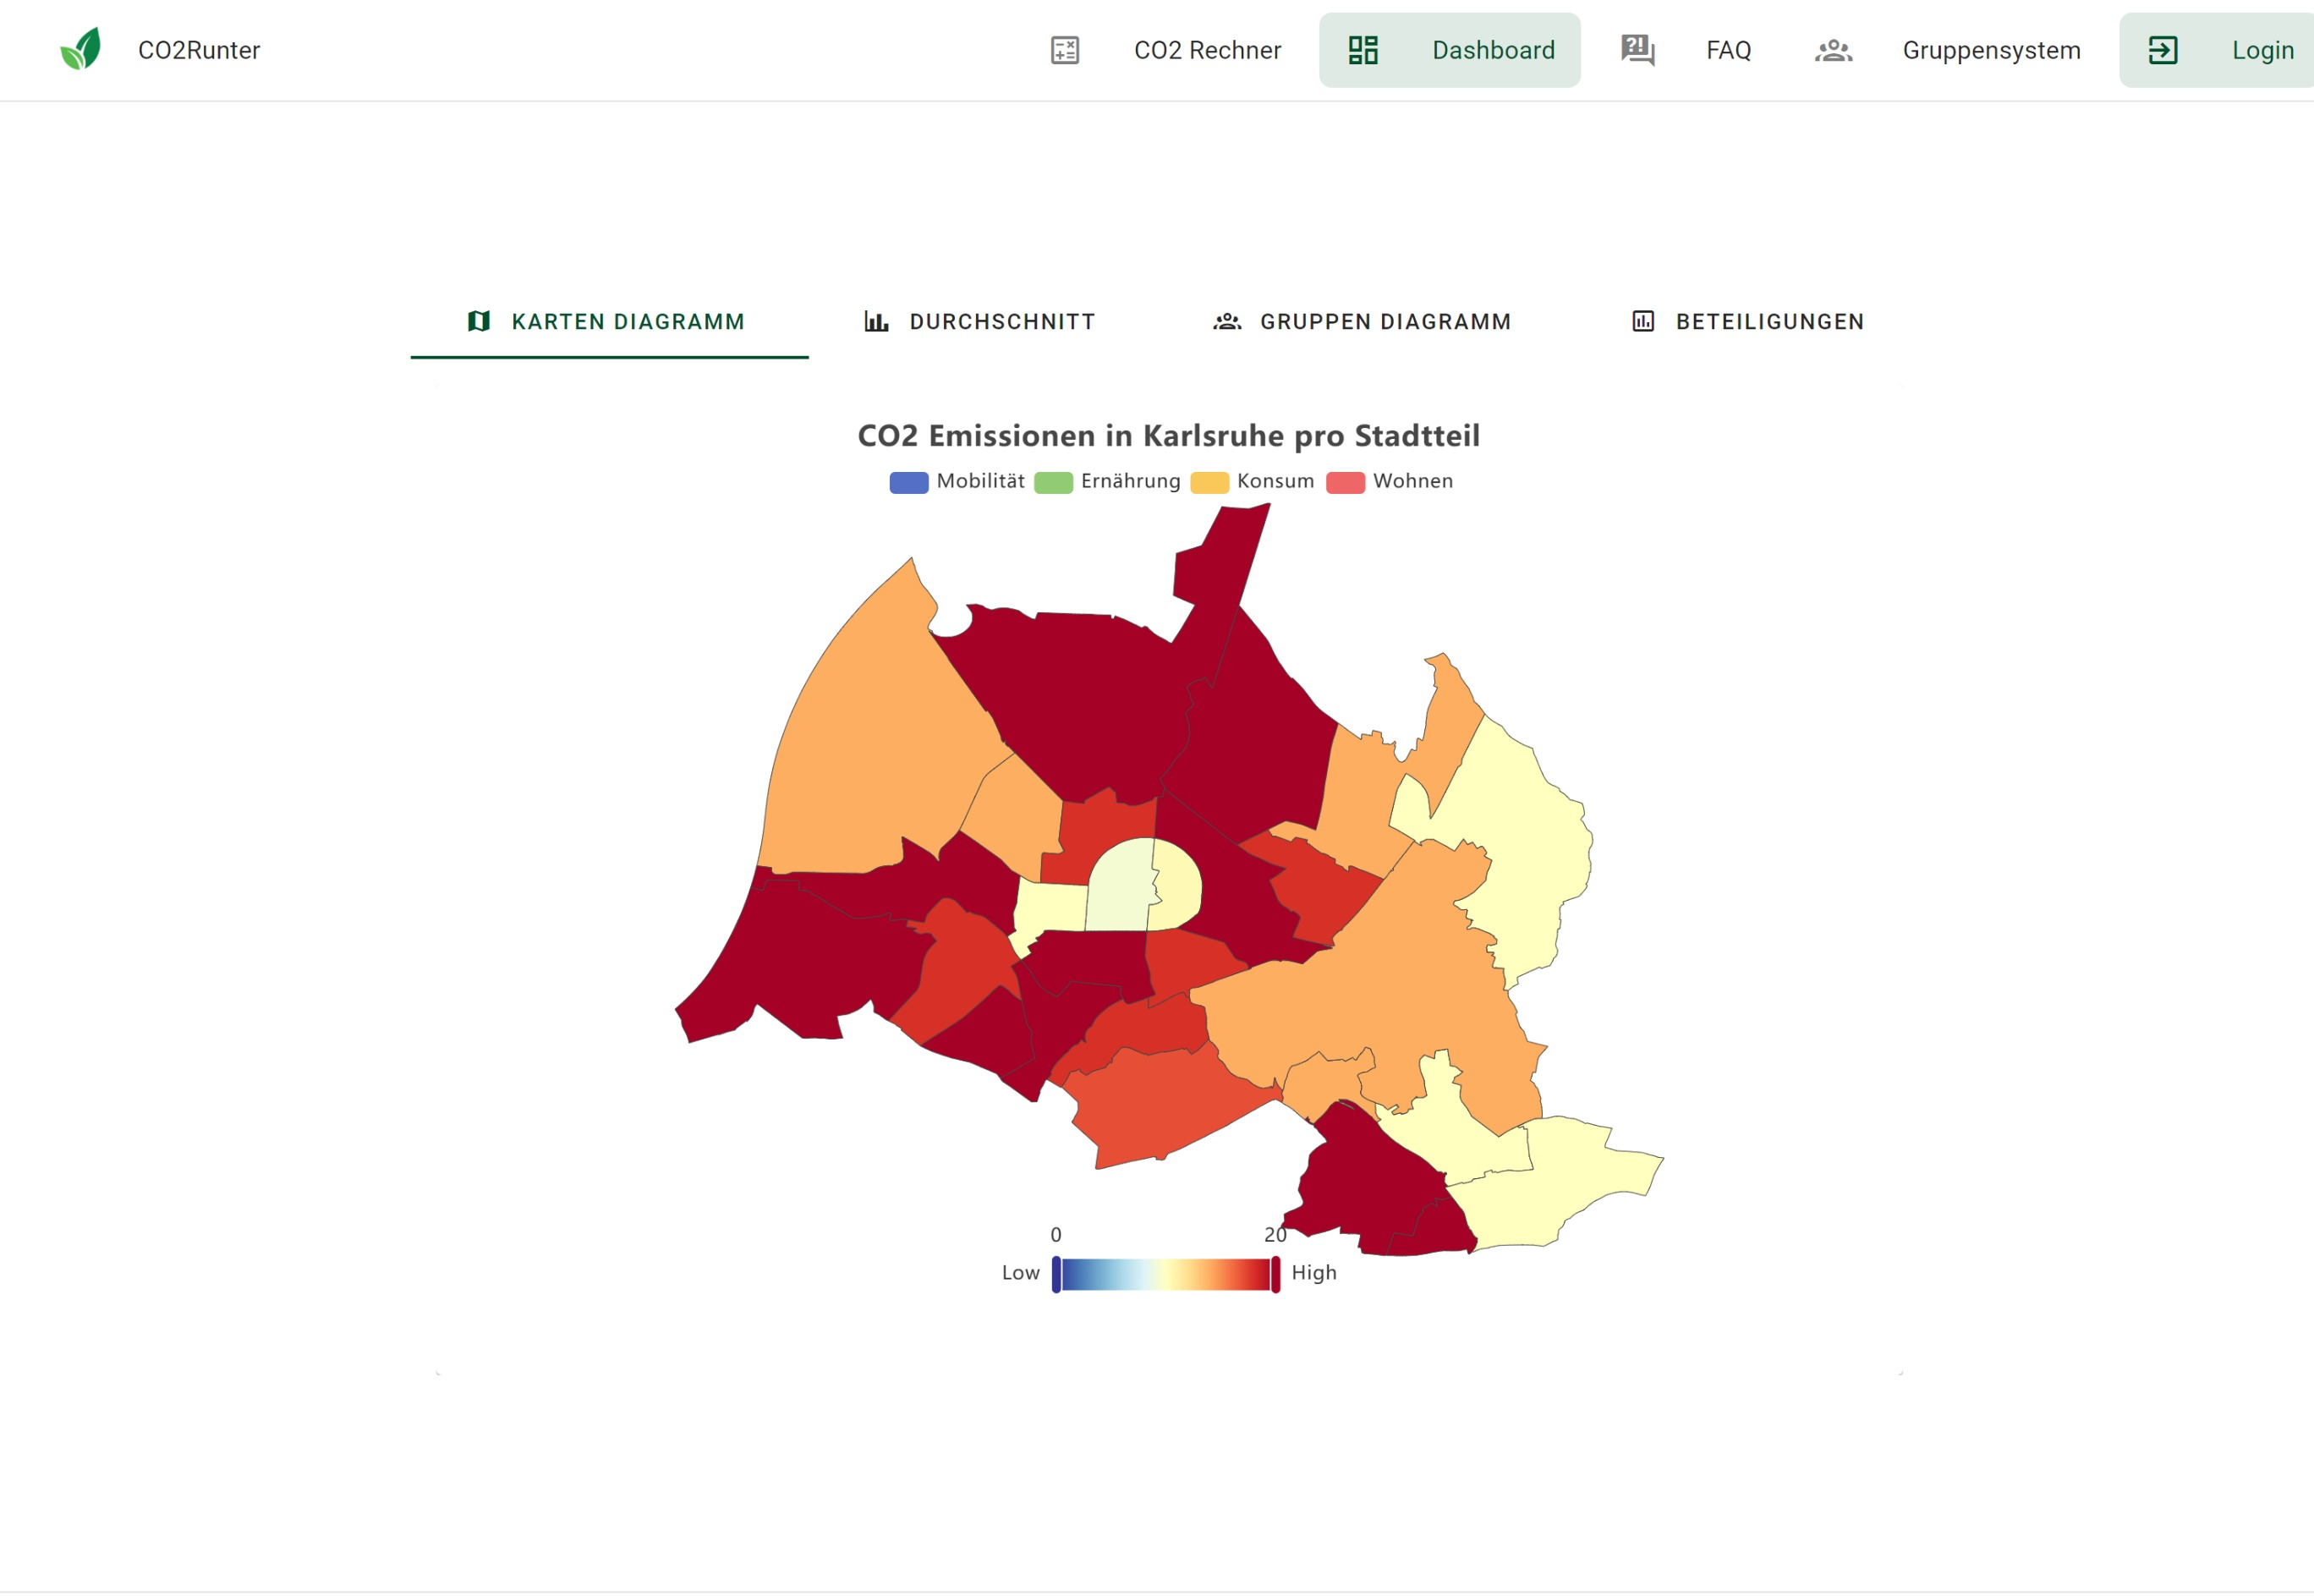
\includegraphics[width=1\textwidth]{images/06/Dashboard-Design.jpeg}
    \caption{Kartendiagramm des Dashboards in der neuen Webseite}
    \label{fig:new-co2runter-dashboard-design}
\end{figure}

\section{Das neue Gruppensystem}

Eine essentielle Funktion der alten Webseite war die Funktion, sich in Gruppen zusammenzuschließen und gemeinsam den CO2-Fußabdruck der Gruppe zu messen und sich gegenseitig zu motivieren, diesen zu reduzieren. Um die \textbf{Anforderung [R17]} zu erfüllen, wurde das Gruppensystem in die neue Webseite integriert und verbessert. Das Gruppensystem besteht aus mehreren Komponenten, die jeweils für einen bestimmten Teil des Gruppensystems verantwortlich sind.



\section{FAQ-Seite}

Und zu guter Letzt wurde noch eine FAQ-Seite der neuen CO2-Runter Webseite hinzugefügt. Der Hintergrund dafür bestand darin, dass es bisher keine Möglichkeit gab, NutzerInnen Informationen zu geben, die nicht direkt mit dem CO2-Rechner oder dem Dashboard zu tun haben. Dadurch will man die Anforderung \textbf{[R18]} erfüllen.

Die FAQ-Seite soll NutzerInnen die Möglichkeit geben, Antworten auf häufig gestellte Fragen zu finden und zusätzlich eine Literaturliste enthalten, die die NutzerInnen nutzen können, um sich weiter zu informieren.

% TODO: Diese Literaturen werden außderdem auch genutzt um beim CO2-Rechner Tips und Tricks anzuzeigen, die den Nutzern helfen können ihren CO2-Fußabdruck zu reduzieren.

Die Implementierung dieser Seite ist relativ einfach, da es sich um eine statische Seite handelt. Die Daten für die FAQ-Seite werden aus einer \acs{JSON}-Datei abgerufen und entsprechend angepasst, um die FAQ-Seite zu erstellen. Hierfür wurden viele Designaspekte übernommen, die bereits auf der Landing Page verwendet wurden. Das Einzige Neue ist die Literaturliste, die durch eine Tabelle realisiert wurde. Hierfür wird lediglich die \acs{JSON}-Datei abgerufen und die Daten in die Tabelle eingefügt. Dies geschieht wie folgt:

\begin{lstlisting}[language={JavaScript}, caption={Laden der Literaturliste}]
<v-data-table
    v-model:page="page"
    :headers="headers"
    :items="LiteratureSources"
    :search="search"
>...</v-data-table>
\end{lstlisting}

Die Literaturliste wird in einer Tabelle dargestellt, die es den NutzerInnen ermöglicht, die Literaturquellen zu durchsuchen und auf die Quellen zuzugreifen. Die Tabelle enthält eine Spalte für den Titel der Quelle, eine Spalte für den Autor, eine Spalte für das Erscheinungsjahr und eine Spalte für den Link zur Quelle. Die Tabelle ist durchsuchbar und paginiert, um die Benutzerfreundlichkeit zu verbessern.

Alle Literaturelemente befinden sich in der \textbf{LiteratureSources}-Variable, die in einer separaten TypeScript-Datei definiert wurde. Dabei handelt es sich um ein Array von Objekten, die die Literaturquellen repräsentieren.

\begin{lstlisting}[language={JavaScript}, caption={Literaturelemente}]
export default const literatureSources: LiteratureSource[] = [
    {
        title: 'Test Title of a Book',
        author: 'Test Name',
        publisher: 'Test Publisher',
        publicationYear: '2019',
        url: 'http://example.com/test-title-of-a-book',
    },
];
\end{lstlisting}

Das finale Design der FAQ-Seite sieht sehr modern und übersichtlich aus und lädt den NutzerInnen dazu ein, sich weiter zu informieren.

\begin{figure}[H]
    \centering
    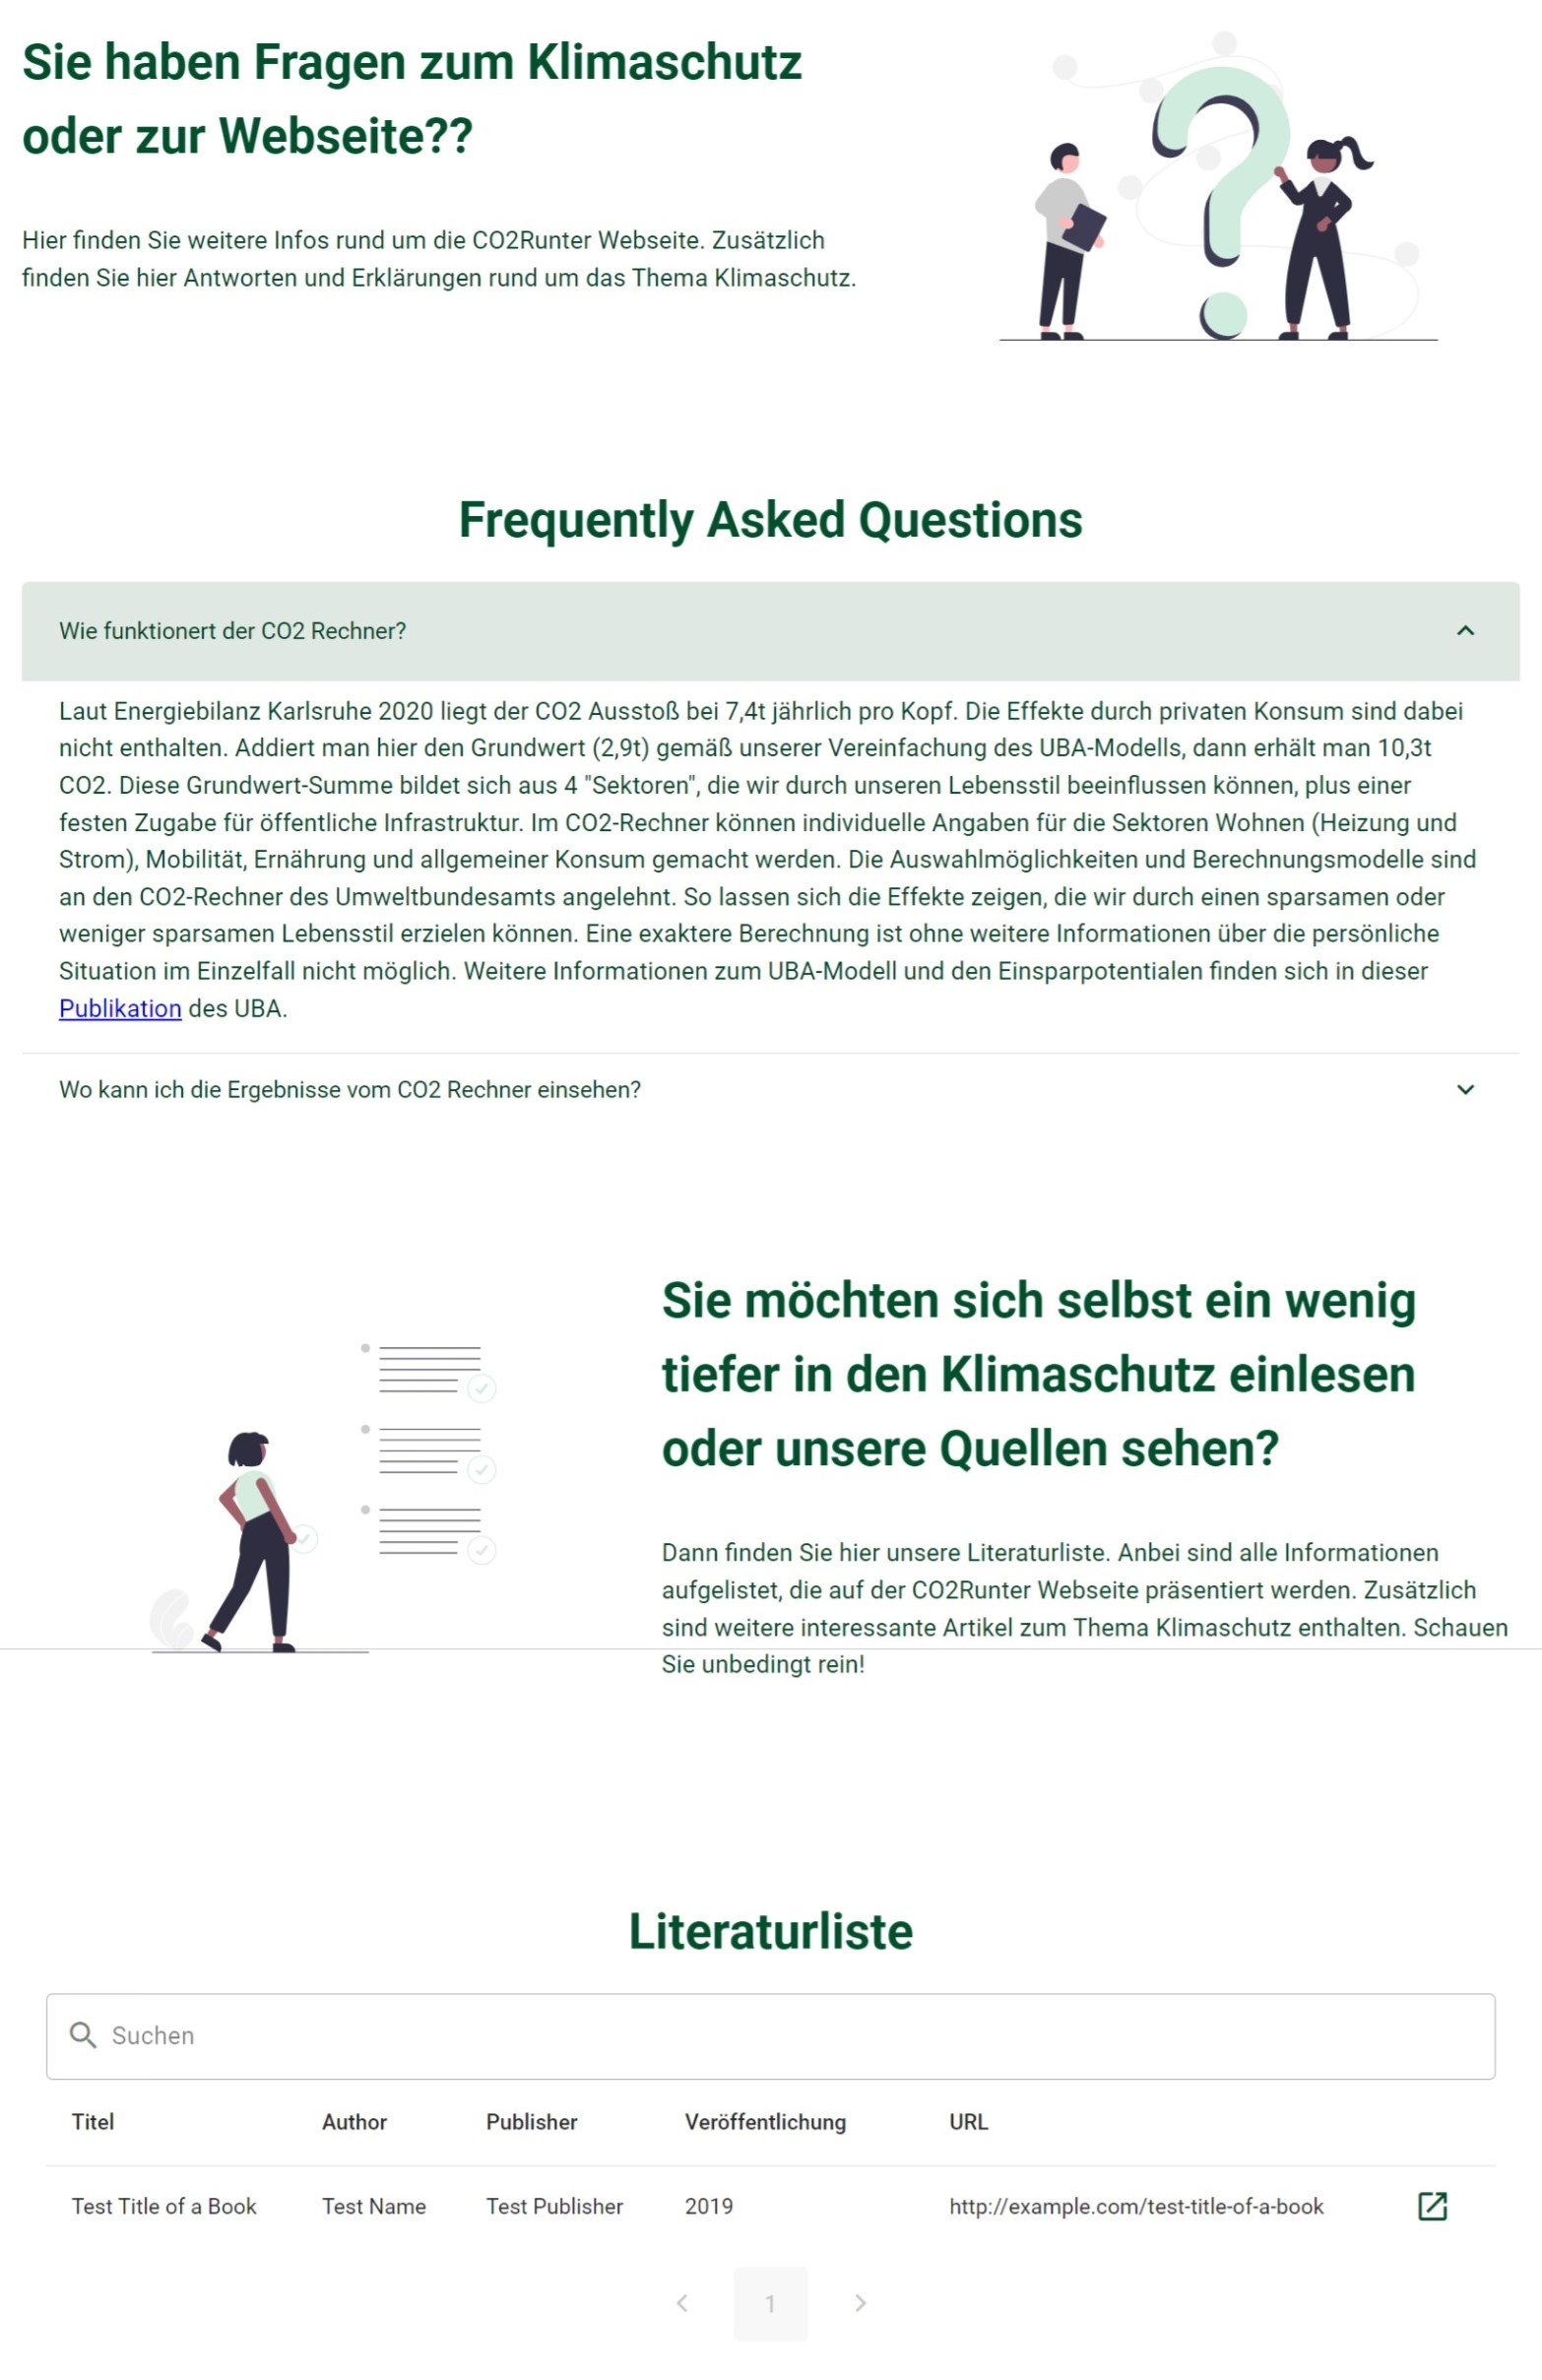
\includegraphics[width=0.8\textwidth]{images/06/FAQ-Design.jpeg}
    \caption{Design der FAQ-Seite der neuen Webseite}
    \label{fig:new-co2runter-faq-design}
\end{figure}

% Überleitung ins nächste Kapitel

Nachdem die neue Webseite erfolgreich implementiert wurde, wird im nächsten Kapitel noch einmal alles zusammengefasst und ein Fazit über die Arbeit und die Ergebnisse gezogen.
